\documentclass[../report.tex]{subfiles}
\begin{document}
\graphicspath{{img/}{../img/}}

\section{The precedence network}
%Which question does this cover / introduction
In order to examine how to balance estimated time with available time to reach a satisfying product by a set deadline, different methods for planning will be investigated. This section will cover The Precedence Network, which is a method for planning a project's activities and their relation.

The Precedence Network represents activities as nodes and the links between these nodes represent precedence requirements. Each activity has a duration, and time flows from left to right. This allows us to perform the \textit{forward pass} and the \textit{backward pass} in order to identify the \textit{critical path}.

	%Identify activities (WBS)
In the activity-based approach all activities that the project is thought to involve are identified. Each activity is estimated before adding it to a node. For now the node only has a \textbf{duration} and a \textbf{label} describing the activity.

	%Build the network
\begin{figure}[H]
\centering
	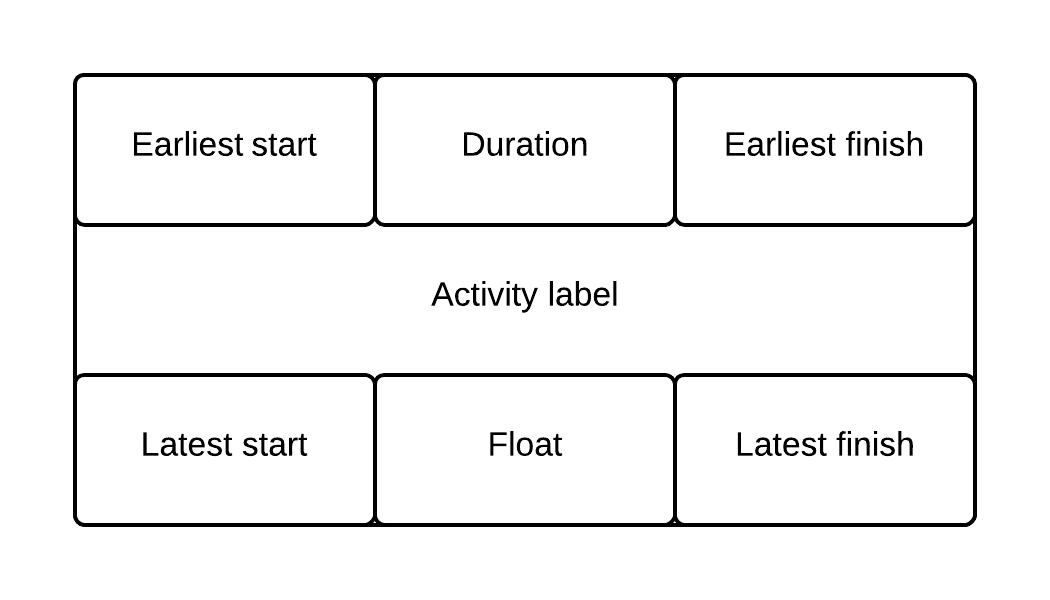
\includegraphics[scale=0.12]{networkNode.png}
\caption{A node in the network}
\end{figure}

Once every activity has been added to a node, the precedence network is created by placing the nodes (activities) in the order of which they are to occur with lines between for representing their dependencies.

	%The forward pass
At this point, the \textit{forward pass} can be executed. This is done by following every path from the start node to the finish node. The \textbf{earliest start} is calculated and filled out by summing up the duration of all prior activities (note that some activities can be executed in parallel, and in this case only the activity with the highest duration is added) while the \textbf{earliest finish} is calculated by adding the current activity's duration to the earliest start.

	%The backward pass
The \textit{backward pass} is, as the name suggests, the opposite. The path from the finish node to the start node is followed, and the \textbf{latest finish} is found by setting the finish node's latest finish to the same as the earliest finish and moving backward. The \textbf{latest start} is found by subtracting the duration of an activity from the latest finish.

The \textbf{float} is the difference between the earliest start and the latest start of a node. This means that if the float is 0, the activity is critical and any delay in the activity will cause a delay of the entire project.

	%Identify the critical path
The critical path is the path in the precedence network where all activities on the path have a float of 0. 

	%A precedence network of our project
//Insert a precedence network of our target project

%Comparison
//Compare this with other planning tools

\end{document}